\documentclass[12pt, a4paper, oneside]{article}
\usepackage{graphicx}
\usepackage{arial}
\renewcommand{\familydefault}{\sfdefault}
\usepackage[T1]{fontenc}
\usepackage[polish]{babel}
\usepackage[utf8]{inputenc}
\usepackage{lmodern}
\usepackage[left=2cm,right=2cm,top=2cm,bottom=2cm]{geometry}
\selectlanguage{polish}
\usepackage{booktabs, multicol, multirow}
\usepackage{longtable}
\usepackage{textcomp}
\usepackage{slashbox}
\begin{document}
\section{Wstęp}
\indent\indent Podczas laboratorium badane są przepustowości standardów IEEE 802.11b oraz 802.11g. Odnoszą się one do warstwy fizycznej (PHY) oraz podwarstwy kontroli dostępu do medium (MAC) w~warstwie łącza modelu ISO OSI. Oba standardy zostały w~pełni ukończone - ich rozwój nie jest kontynuowany, a obecnie pierwszy z nich praktycznie całkowicie odszedł z użycia. Dla 802.11b zdefiniowano 13 kanałów (14 poza Europą) w paśmie 2,4 - 2,4835 GHz. Każdy z~kanałów ma szerokość 22 MHz. Częstotliwości środkowe kanałów przesunięte są względem siebie o 5 MHz, co powoduje nakładanie się wielu kanałów. Jedynie kanały 1, 6 oraz 11 są od siebie oddalone na tyle, że nie występuje ich nakładanie się, a nawet występuje odstęp 3 MHz pomiędzy granicznymi częstotliwościami kanałów.\\
\indent IEEE 802.11b posiada dwie metody rozpraszania widma pozwalające na osiąganie różnych przepływności. Pierwsza z nich to DSSS (Direct Sequence Spread Spectrum), polegająca na mnożeniu sygnału przez szybkozmienny sygnał kodowy. Pozwala to na rozproszenie (poszerzenie) widma sygnału i tym samym uniknięcie zakłóceń wąskopasmowych. Przy DSSS stosowane są modulacje DBPSK pozwalająca osiągnąć przepływność 1 Mbps oraz DQPSK zwiększająca przepływność do 2 Mbps. Większe szybkości udało się osiągnąć poprzez zastosowanie CCK (Complementary Code Keying), które działa jak DSSS, jednak wykorzystuje sprawniejsze ciągi kodowe. Pozwala to na osiągnięcie 5.5 Mbps przy modulacji DBPSK oraz 11 Mbps dla DQPSK.\\
\indent IEEE 802.11g można traktować jako rozwinięcie standardu 802.11b. Dostępne są szybkości 1,~2,~5,5, 11 Mbps realizowane jak w 802.11b oraz dzięki zastosowaniu Orthogonal Frequency Division Multiplexing (OFDM) i innych modulacji: 6, 9 Mbps z modulacją BPSK, 12, 18 Mbps z~modulacją QPSK, 24, 36 Mbps modulowane z użyciem 16-QAM oraz 48 i 54 Mbps przy wykorzystaniu modulacji 64-QAM.
\begin{figure}[h!]
\centering
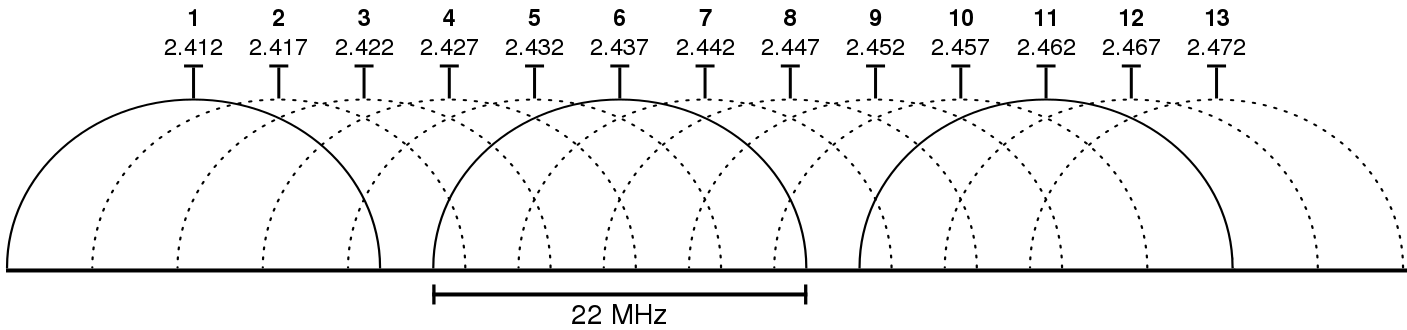
\includegraphics[scale=0.45]{pics/f2.png}
\caption{Schemat kanałów dostępnych w Europie dla IEEE 802.11b/g}
\end{figure}\\
\indent W trybie kompatybilności z 802.11b preambuła i nagłówek nadawane są z szybkością 1 Mbps. W trybie ,,g only'' preambuła i nagłówek przesyłane są z szybkością 6 Mbps. Wpływ długości preambuły na przepływność podlega badaniu podczas laboratorium.\\
\indent Oba standardy implementują Automatic Rate Fallback (ARF), co pozwala na automatyczną adaptację szybkości w zależności od minimalnej mocy odebranej. Zmniejszenie szybkości transmisji przy obniżeniu się poziomu mocy pozwala na utrzymanie stałej stopy błędów Bit Error Rate (BER) na poziomie 10$^{-5}$. W przypadku niskiego poziomu mocy i wymuszonej wysokiej szybkości transmisji, stopa błędów może ulec gwałtownemu wzrostowi, co obniży jakość transmisji i będzie wymuszało kolejne retransmisje obniżające rzeczywistą przepływność.\\
\indent W dalszej części laboratorium badany jest wpływ długości pakietu UDP na przepustowość. Na tym etapie szybkość ustawiona jest na maksymalną teoretyczną wartość równą 54 Mbps. Urządzenie po odebraniu określa czy otrzymany z wyższej warstwy pakiet może zostać przesłany w jednej ramce. Maksymalna długość wynosi 2 346 B. Jeśli nie, to następuje jego fragmentacja. Zgodnie z~protokołem CSMA/CA i DCF - rozproszoną funkcją koordynującą (w praktyce jedynie ta jest implementowana w urządzeniach powszechnego użytku) urządzenie zgłasza gotowość przez wysłanie pakietu Ready To Send (RTS). Jeśli po okresie Short Interframe Space (SIFS) otrzyma pakiet Clear To Send (CTS), to rozpoczyna transmisję ramek. Po każdej z nich, po odczekaniu SISF, oczekuje na potwierdzenie ACK od odbiorcy. Następnie po odczekaniu kolejnego SISF, wysyła następny fragment nie rywalizując ponownie o dostęp do medium. Po otrzymaniu ACK po ostatnim fragmencie czeka okres Distributed IFS (DIFS).\\
\indent Podobne pomiary przeprowadza się dla wpływu fragmentacji warstwy MAC na przepustowość. Powyżej zadanego rozmiaru, każda ramka jest dzielona i przesyłana we fragmentach. Większa ilość przesyłanych ramek wymaga częstszego oczekiwania na potwierdzenie ACK. Jednak dzięki takiemu dzieleniu i ponownemu łączeniu po stronie odbiorcy można uzyskać mniejszą ilość błędów transmisji.
\indent Badaniu podlega także wpływ procedury RTS/CTS na przepustowość. RTS jest wysyłany, kiedy stacja chce zacząć nadawać. Inne stacje w zasięgu wstrzymują się wtedy z rozpoczęciem transmisji, a nadawca oczekuje na CTS od adresata RTS. Odbiorca wysyłając CTS informuje stacje w swoim zasięgu o transmisji, którą będzie prowadził. Wykorzystanie RTS/CTS pozwala na uniknięcie zjawiska stacji ukrytej.\\
\indent Omawiane standardy pozwalają także na uwierzytelnianie kluczem współdzielonym Wired Equivalent Privacy (WEP). Jest to standard szyfrowania powstały w 1999r. i obecnie bardzo prosty do złamania. Klucz 40 lub 104 bitowy łączony jest z 24 bitowym wektorem inicjującym. Tak otrzymany 64 lub 128 bitowy klucz podawany jest na wejście generatora liczb pseudolosowych, który na tej podstawie generuje pseudolosową sekwencję kluczową, która wykorzystywana jest do wykonania XOR zarówno z wektorem integralności jak i danymi. Metoda ta pozwala na otrzymanie 4 różnych kluczy.
\section{Sprzęt i konfiguracja}
\indent\indent Podczas laboratorium zestawiono sieć złożoną z:
\begin{itemize}
\item laptopa (192.168.1.110/24) łączącego się bezprzewodowo z punktem dostępowym (AP),
\item laptopa (192.168.1.4/24) połączonego kablem Ethernet z AP,
\item AP (192.168.1.1/24).
\end{itemize}
\begin{figure}[h!]
\centering
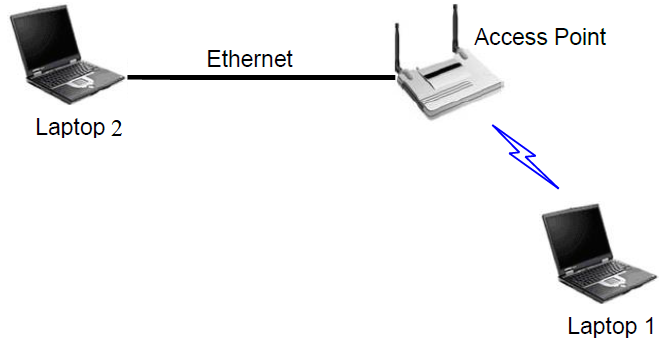
\includegraphics[scale=0.4]{pics/f1.png}
\caption{Stanowisko laboratoryjne}
\end{figure}
\clearpage
\section{Wyniki pomiarów}
\section{Wnioski}
\end{document}